\chapter{Méthodes de travail}
Mimesis Republic utilise une méthode de travail agile, appelée Scrum.
\section{Méthode agile Scrum}
Scrum est une méthode agile dédiée à la gestion de projets.
Parmi les méthodes de développement agiles existantes, on peut citer :
\begin{itemize}
\item Scrum
\item Extreme Programming
\item Adaptive Software Development (ASD)
\item Dynamic System Development Method (DSDM)\\
\end{itemize}
Le terme Scrum est emprunté au rugby et signifie mêlée. Ce processus
s'articule en effet autour d'une équipe soudée, qui cherche à atteindre un but,
comme c'est le cas en rugby pour avancer avec le ballon pendant une mêlée.\\
\subsection{Sprints}
Scrum est un processus itératif : les itérations sont appelées des sprints et
durent entre 2 et 4 semaines.
Chez Mimesis Republic, les sprints durent habituellement 2 semaines.
\begin{figure}[H]
  \begin{center}
    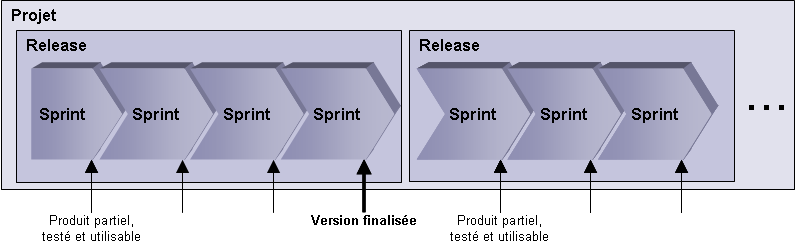
\includegraphics[width=\textwidth]{planification_scrum.png}
  \end{center}
  %% \caption{Exemple de planification Scrum}
\end{figure}

\clearpage
\subsection{Issues}
Avant de commencer un sprint, on lui associe une liste de fonctionnalités qui
devront être réalisées, tirées du backlog de produit (cf. Schéma Vue synthétique
du processus Scrum).\\
Ces fonctionnalités sont sélectionnées pour être implémentées dans ce sprint.\\

Chaque fonctionnalité est découpée par l'équipe en tâches élémentaires de
quelques heures et vont dans le backlog de sprint. Ces tâches élémentaires sont
appelées des \textbf{issues} et peuvent être consultées à tout moment par les
programmeurs.\\

L'image ci dessous présente la liste des issues qui m'ont été
assignées. \\
Chaque membre de l'équipe peut les consulter et y ajouter un
commentaire, pour discuter de l'implémentation ou pour proposer des
solutions possibles.

\begin{figure}[H]
  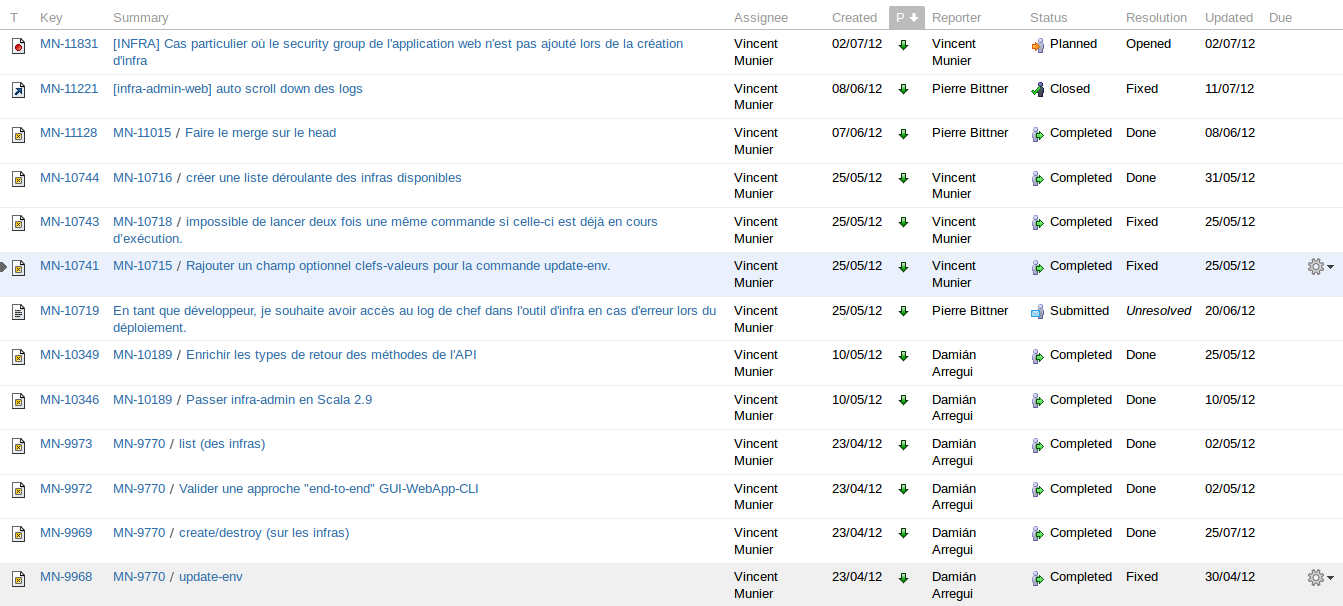
\includegraphics[width=\textwidth]{mes-issues.png}
  \caption{Liste des issues qui m'ont été assignées}
\end{figure}

\clearpage

Une issue est la description très courte d'un besoin utilisateur.\\
Dans l'exemple ci-dessous, nous pouvons retrouver les différentes informations
attachées à une issue. \\
Nous pouvons retrouver la date de création, le nombre d'heures estimé, le nombre
d'heures loguées et bien d'autres informations.\\

\begin{figure}[H]
  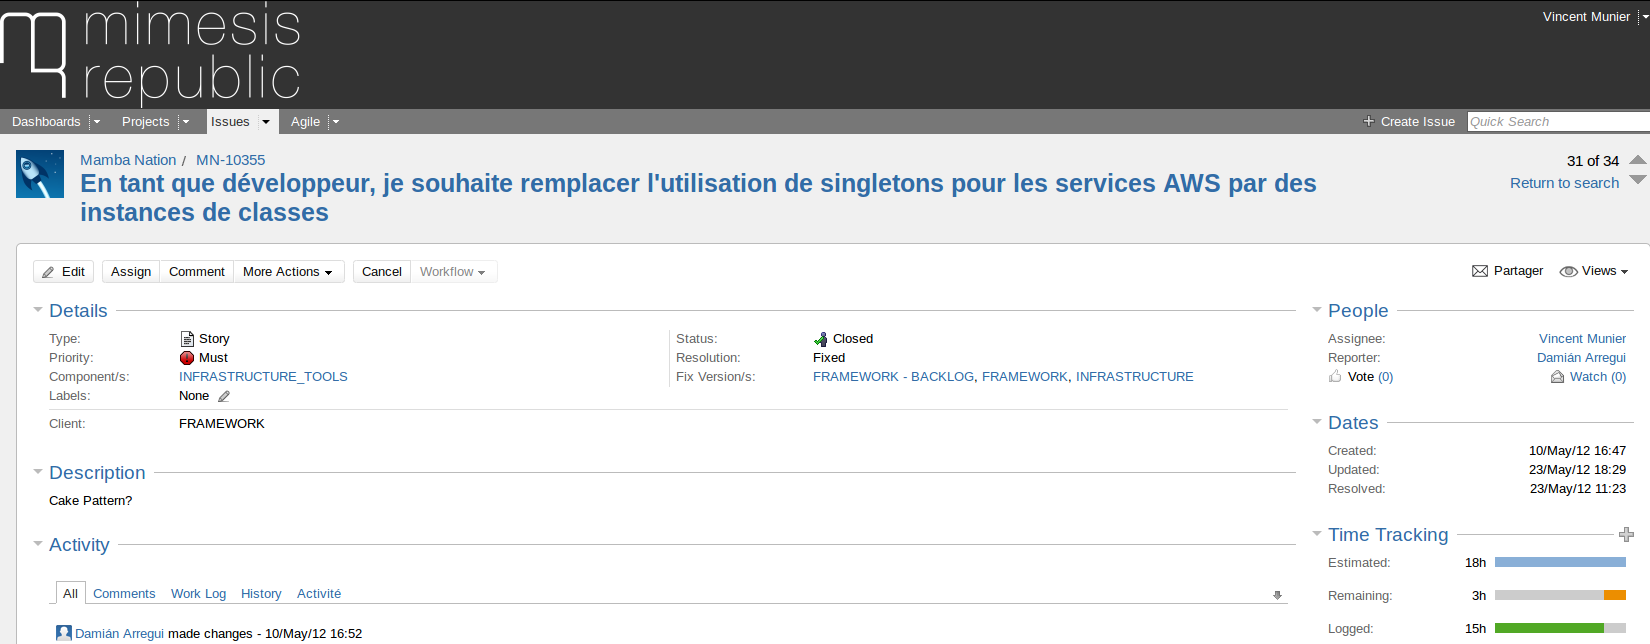
\includegraphics[width=\textwidth]{issue-MN-10355.png}
  \caption{Exemple d'issue qui m'a été attribué}
\end{figure}

Ce découpage de tâches de courtes durées est un des gros points forts de la
méthodologie agile Scrum.\\
En effet, il permet d'avoir un système testable qui peut être livré au client à
chaque instant. Bien sur, nous devons prévenir le client que telle
fonctionnalité n'est pas encore implémentée.\\
Mais le client peut ainsi nous faire des retours sur ce qu'il en pense, le plus
régulièrement possible.\\
En cas de problèmes, il est bien plus facile de faire des interventions rapides
que si le client donnait son avis tous les six mois.\\
Il peut également décider à tout instant de mettre son produit en production
s'il le souhaite.

\subsection{Réunions}
\subsubsection{Réunion chaque jour}
Chaque journée de travail commence par une réunion de 15 minutes maximum appelée
standup (Daily standup).\\

Le ScrumMaster donne la parole à chaque membre de l'équipe.\\
À tour de rôle,  nous devons répondre à 3 questions :
\begin{itemize}
\item Qu'est-ce que j'ai fait hier ?
\item Qu'est-ce que je compte faire aujourd'hui ?
\item Quelles sont les difficultés que je rencontre ?\\
\end{itemize}
L'équipe se met ensuite au travail, elle travaille dans une même pièce.

\subsubsection{Réunion entre deux sprints}
À la fin du sprint, tout le monde se regroupe pour effectuer une réunion qui se
déroule en deux étapes :
\begin{itemize}
\item La revue de sprint (sauf si c'est le premier sprint)
\item La planification du prochain sprint\\
\end{itemize}

La durée de cette réunion est d'environ quatre heures.\\\\
\textit{\underline{Revue du sprint précédent}}\\

Le Scrum Master commence par faire une présentation de ce qui était attendu pour
ce sprint.\\
Puis il énonce les fonctionnalités qui ont été réellement implémentées, groupées
par programmeur.\\
Le Scrum Master donne ainsi la parole à chaque membre de l'équipe, pour qu'il
donne un retour d'expérience, les tâches qu'il a accomplies avec succès, les
imprévus qu'il a rencontrés.\\\\
\textit{\underline{Planification du sprint à venir}}\\

La réunion de planification consiste à définir d'abord
un but pour le sprint, puis à choisir les fonctionnalités de produit qui seront
réalisées dans ce sprint. \\

Dans un second temps, l'équipe décompose chaque fonctionnalité de produit en
liste de tâches (items du backlog du sprint), puis estime chaque tâche en
nombre d'heures. 

\begin{figure}[H]
  \begin{center}
    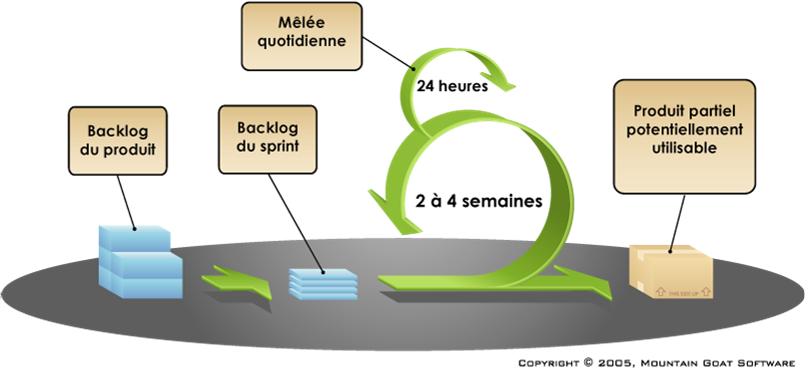
\includegraphics[width=\textwidth]{scrum.png}  
  \end{center}
  \caption{Vue synthétique du processus Scrum}  
  \label{scrumsynthese}
\end{figure}

\newpage
\subsection{Glossaire}

\begin{itemize}
\item[]\textbf{Backlog}

  Liste ordonnée de toutes les choses à faire. Il y a le backlog de produit qui
  énumère les exigences avec le point de vue du client et le backlog de sprint qui
  contient les tâches de l'équipe. \\

\item[]\textbf{Directeur de produit / Product owner}

  Le représentant des clients. Littéralement le propriétaire du produit.\\

\item[]\textbf{Release}

  Une release correspond à la livraison d'une version. Par habitude, on parle de
  release pour considérer la période de temps qui va du début du travail sur cette
  version jusqu'à sa livraison et qui passe par une série de sprints
  successifs. \\

\item[]\textbf{Scrum}

  Scrum c'est la méthode mais c'est aussi le nom usuel de la réunion quotidienne
  limitée à un quart d'heure. \\

\item[]\textbf{Sprint}

  Bloc de temps aboutissant à créer un incrément du produit potentiellement
  livrable. C'est le terme utilisé dans Scrum pour itération. Aux débuts de Scrum,
  un sprint durait 30 jours. La pratique actuelle est de 2 à 4 semaines.\\

\item[]\textbf{Scrum Master}

  Il dirige les réunions scrum. Il s'assure que le projet avance comme prévu.\\
\end{itemize}



